\documentclass[12pt]{article}
\usepackage{amsmath}
\usepackage{graphicx,psfrag,epsf,comment}
\usepackage{enumerate}
\usepackage{natbib}
\usepackage{url} % not crucial - just used below for the URL 
\bibliographystyle{chicago}


%\pdfminorversion=4
% NOTE: To produce blinded version, replace "0" with "1" below.
\newcommand{\blind}{0}

% DON'T change margins - should be 1 inch all around.
\addtolength{\oddsidemargin}{-.5in}%
\addtolength{\evensidemargin}{-.5in}%
\addtolength{\textwidth}{1in}%
\addtolength{\textheight}{1.3in}%
\addtolength{\topmargin}{-.8in}%

\newcommand{\logit}{\mathrm{lgt}}
\newcommand{\I}{\mathrm{I}}
\newcommand{\E}{\mathrm{E}}
\newcommand{\p}{\mathrm{P}}
\newcommand{\e}{\mathrm{e}}
\renewcommand{\o}{\omega}
\newcommand{\vecm}{\mathrm{vec}}
\newcommand{\kp}{\otimes}
\newcommand{\diag}{\mathrm{diag}}
\newcommand{\cov}{\mathrm{cov}}
\newcommand{\eps}{\epsilon}
\newcommand{\ep}{\varepsilon}
\newcommand{\obdots}{\ddots}    % change this later
\newcommand{\Ex}{{\cal E}}
\newcommand{\Exd}{\Ex_d}
\newcommand{\Es}{\E_\phi}
\newcommand{\rat}{{\frac{c_{ij}}{c_{i,j-1}}}}
\newcommand{\rmu}{m}
\newcommand{\rsig}{\nu}
\newcommand{\fd}{\mu}
\newcommand{\tr}{\mathrm{tr}}
\newcommand{\cor}{\mathrm{cor}}
\newcommand{\bx}[1]{\ensuremath{\overline{#1}|}}
\newcommand{\an}[1]{\ensuremath{a_{\bx{#1}}}}

\newcommand{\bi}{\begin{itemize}}
\newcommand{\ei}{\end{itemize}}

\renewcommand{\i}{\item}
\newcommand{\sr}{\ensuremath{\mathrm{SRISK}}}
\newcommand{\cs}{\ensuremath{\mathrm{CS}}}
\newcommand{\cri}{\ensuremath{\mathrm{Crisis}}}
\newcommand{\var}{\ensuremath{\mathrm{VaR}}}
\newcommand{\covar}{\ensuremath{\mathrm{CoVaR}}}
\newcommand{\med}{\ensuremath{\mathrm{m}}}
\newcommand{\de}{\mathrm{d}}
\renewcommand{\v}{\ensuremath{\mathrm{v}_q}}
\newcommand{\m}{\ensuremath{\mathrm{m}}}
\newcommand{\tvar}{\ensuremath{\mathrm{TVaR}}}
\renewcommand{\c}{\ensuremath{\mathrm{CoVaR_q}}}
\renewcommand{\v}{\ensuremath{\mathrm{VaR}_q}}



\newcommand{\eref}[1]{(\ref{#1})}
\newcommand{\fref}[1]{Figure \ref{#1}}
\newcommand{\sref}[1]{\S\ref{#1}}
\newcommand{\tref}[1]{Table \ref{#1}}
\newcommand{\aref}[1]{Appendix \ref{#1}}




\newcommand{\cq}{\ , \qquad}
\renewcommand{\P}{\mathrm{P}}
\newcommand{\Q}{\mathrm{Q}}

\newcommand{\Vx}{{\cal V}}
\newcommand{\be}[1]{\begin{equation}\label{#1}}
\newcommand{\ee}{\end{equation}}



\begin{document}

%\bibliographystyle{natbib}

\def\spacingset#1{\renewcommand{\baselinestretch}%
{#1}\small\normalsize} \spacingset{1}


%%%%%%%%%%%%%%%%%%%%%%%%%%%%%%%%%%%%%%%%%%%%%%%%%%%%%%%%%%%%%%%%%%%%%%%%%%%%%%

\if0\blind
{
  \title{\bf Measuring background and systemic risk using financial time series}
  \author{Piet de Jong\thanks{
    The authors gratefully acknowledge CIFR, the Centre of International Financial Regulation for financial support and other assistance.}\hspace{.2cm}\\
    Department of Applied Finance and Actuarial Studies, Macquarie University\\
    and \\
    Geoffrey Loudon\\
    Department of Applied Finance and Actuarial Studies, Macquarie University\\
    and\\
    Weihao Choo\\
    Department of Applied Finance and Actuarial Studies, Macquarie University}
  \maketitle
} \fi

\if1\blind
{
  \bigskip
  \bigskip
  \bigskip
  \begin{center}
    {\LARGE\bf Measuring background and systemic risk using financial time series}
\end{center}
  \medskip
} \fi

\bigskip
\begin{abstract}
This article refines and extends  SRISK methodology recently proposed in the literature.  The refinement is to define systemic risk in terms of a put on the Basel shortfall.  Background and systemic stress  of a firm are defined as unconditional, and departure from unconditional  expectation, of the put, the latter when a hypothetical systemic stress is applied.  Systemic stress is defined in terms of a random variable and can take on variety of forms including alternative scenarios in usual stress testing as well stress driven by the interaction of variables.  Stressor random variables  are chosen by the practitioner.  Stressed expectations are linear, a sector systemic stress is naturally defined as linear in the firm specific systemic stress.      Application is made to Australian financial daily time series data.
\end{abstract}

\noindent%
{\it Keywords:}  Capital shortfall, background risk, Basel put, stressed expectation.
\vfill

\newpage
\spacingset{1.45} % DON'T change the spacing!

Monitoring stresses and systemic risk in the financial system is a key function of macro--prudential regulation. Central banks and other financial regulatory bodies such as the US Financial Stability Oversight Council, the European Systemic Risk Board and the Australian Prudential Regulation Authority [APRA] are concerned with developing and applying early warning quantitative  measures  to warn of potential episodes of heightened systemic risk. Systemic risk has many dimensions. For example, in their influential review paper, \cite{Bisias2012} present a taxonomy of six categories of systemic risk comprising 31 quantitative risk measures. While attempts to gain consensus on a theoretical definition have proved elusive, several empirical measures of systemic risk have been developed and applied with  success.  An important example is the SRISK measure due to \cite{brownlees2015} -- an index that measures the expected capital shortfall of a financial institution conditional on a large and lengthy decline in equity markets. \cite{brownlees2015} show that their SRISK based measures are able to identify systemically important financial firms and are informative about the impact of financial crises on future macro-economic conditions. 

Our paper refines and extends the model of \cite{brownlees2015} in several interesting and important ways. First, we reinterpret their SRISK measure as a put on the expected shortfall using stressed expectation. While they condition on the event of a severe market downturn, we take the stressed expectation of the put value. This enables us to capture the impact of increased return volatility due to stress. Second, we decompose their SRISK measure into background stress and imposed system stress. Background stress is a function of existing volatility and leverage. As these factors increase, background stress rises and this makes the firm more susceptible to systemic risk, regardless of the stress event itself. Third,    
\cite{brownlees2015} condition on an absolute cutoff of arbitrary size and length. We suggest that it is also helpful to specify conditional behaviour in percentile terms relative to current market conditions. This provides a sharper focus on the incremental impact of further stress and allows us to draw stronger implications from SRISK numbers. These extensions provide additional insights into the sources and economic nature of systemic risk. They provide potentially new and improved ways of anticipating episodes of heightened systemic risk. Their practical use can be expected to help regulators monitor systemic risk in a timely fashion to facilitate remedial action where necessary.

% This study aims to extend and apply these techniques particularly in relation to the entities regulated by the Australian Prudential Regulation Authority (APRA). Thus our  broad aim is to develop, implement and bring to bear recent developments in systemic risk measurement and stress testing  on the aims of APRA and the CIFR targeted research areas.   (This needs much more commentary).

While our measures are designed for use in all financial systems, it is of particular interest to test them using the Australian setting for at least two reasons. First, the Australian financial system is dominated by only four banks. In Australia there are four major banks that hold 78\% of the total assets of all Authorised Deposit-taking Institutions in  Australia.\footnote{Based on balances at 31 December 2014 disclosed in APRA's Quarterly Authorised Deposit-taking Institution [ADI] Performance Report for March 2015.} It is therefore obvious that the four majors are systemically important and the remaining ADIs are not so unless stress in one of these minors somehow creates financial contagion to the majors, in an unforeseeable way. Second, the Australian banking system proved to be resilient through the recent global financial crisis [GFC], implying that systemic risk did not reach the extreme levels experienced by other countries where bank failures occurred. Both these features of the Australian system suggest that it may be difficult to find useful additional information about systemic risk by refining quantitative measures like SRISK. Since we are able to show that our measures are informative about systemic risk in Australia, we conjecture that they will provide additional insights elsewhere.  

To demonstrate the nature and usefulness of our measures, we use publicly available daily financial data for the eight Australian banks detailed in \tref{eightbanks} spanning the period from  3 April 2000 through to 1 December 2014.  The data is described in detail in \aref{data}.  Prices, adjusted for dividends are plotted in \fref{prices}.  Prices are combined with number of shares to derive total equity. Total debt for each firm is also collected from annual accounting reports. % (Should these be plotted? No, not informative;  leverage ratio plots are sufficient). 

Remaining sections are structured as follows. Section \ref{litrev} briefly discusses some related literature. Section \ref{capshort} and \ref{futshort} define current and future  capital shortfall similarly as \cite{brownlees2015} under a simplistic Basel II regulatory framework. The definition of systemic risk used by \cite{brownlees2015} is discussed in \sref{srisk}, and is refined, extended and illustrated \sref{improve} to \sref{estimate}. Section \ref{marketstress} discusses specific stress examples which extend beyond \cite{brownlees2015}. Applications to Australian bank data are discussed in \sref{simulate} and \sref{simulate1}. Section \ref{aggregate} and \ref{aggregate1} discuss how stresses are combined across firms with and without allowance for merging or diversification. Section \ref{monitoring} displays system stress calculations as they would proceed in real time. Generalised stresses are outlined in \sref{genstress}.  Section \ref{riskmethod} offers an alternative modelling approach, based on assets. Section \ref{comparison} summarises differences between proposed stress measurement in this paper with that of 
\cite{brownlees2015}. Section \ref{conclude} concludes.

\begin{table}[htdp]
\label{banks}\caption{Major and minor Australian banks}\label{eightbanks}
\begin{center}
\begin{tabular}{l|l||l|l}
\hline
 \multicolumn{2}{c||}{major}& \multicolumn{2}{c}{minor}\\
 \hline
CBA & Commonwealth Bank  & MQG & Macquarie \\
ANZ & Australia \& New Zealand  & BOQ & Bank of Queensland\\
NAB & National Australia  & BEN & Bendigo and Adelaide \\
WBC & Westpac & ABA& Auswide \\
\hline
\end{tabular}
\end{center}
\end{table}%


\begin{figure}[htbp]
\begin{center}
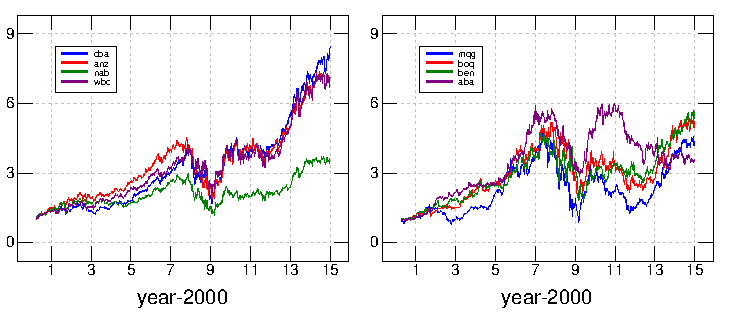
\includegraphics{figures/prices.pdf}
\caption{Stock  prices of four major (left panel) and four minor (right panel) Australian banks from early 2000 through to the end of 2014.  Price series normalised to start at 1.}
\label{prices}
\end{center}
\end{figure}

\section{Literature review}\label{litrev}
Many papers in the finance and economics literature are devoted to the development and application of a variety of quantitative measures of systemic risk or financial stress. \cite{Bisias2012} provide an instructive and qualitative survey of numerous measures in use. \cite{Giglio2015} supply empirical evidence on the ability of many of these measures, both individually and collectively, to provide early warning signals of deterioration in macro-economic conditions. In this section, we provide a selective overview of those measures most closely related to SRISK and its relevance for assessing systemic risk in the financial sector. 

The genesis of SRISK lies in a series of papers including \cite{acharya2012aer}, \cite{acharya2012wp} and \cite{brownlees2010volatility}. In these papers, SRISK is defined as the expected capital shortfall of a financial firm, conditional on a crisis. A crisis is deemed to occur whenever a relevant market index suffers a significant decline over a chosen horizon. SRISK measures require an estimate of the long run marginal expected shortfall [LRMES] which is typically obtained by simulation methods.

\cite{brownlees2015} further develop the empirical methodology to construct SRISK measures. SRISK depends on the firm's size, leverage and its LRMES. The LRMES is obtained by assuming a dynamic process for the joint distribution of firm and market returns. \cite{brownlees2015} use  the standard GARCH-DCC model of \cite{engle2002dynamic} with threshold ARCH volatilities on the basis that this represents a good trade-off between model complexity and prediction accuracy. The LRMES is computed as the Monte Carlo average of simulated multi-period returns,  conditional on the return being worse than the cut-off level chosen to identify a financial crisis. Using a sample of large US financial firms,  \cite{brownlees2015} show the practical usefulness of their measure in three ways: (i) SRISK rankings identify systemically risky US banks during the GFC; (ii) pre-crisis SRISK helps predict capital injections by the Fed Reserve; (iii) aggregate SRISK provides early warning of declines in industrial production and higher unemployment.
     
\cite{Engle2015} extend the model in \cite{brownlees2015} to incorporate global, country and industry effects. This extended model makes effective use of \cite{Engle2014dcb}'s dynamic conditional beta model. Their empirical methods are able to provide information about the relative systemic importance of industry type and country identity. For instance, they find  that systemic risk in Europe during the GFC was predominantly due to banks while France and the UK recorded the largest country-level SRISK numbers. 

\cite{adrian2011covar} propose an alternative measure of systemic risk that emphasises the co-dependence of financial firms and the importance of risk spillovers within the financial sector. They introduce CoVaR$_i$ which computes the Value-at-Risk [VaR] of the entire financial system, conditional on institution $i$ being in distress. Distress is defined as the state where the institution is exactly at its VaR level. \cite{Girardi2013} improve CoVaR by conditioning on the institution being at most at its VaR. This generalisation is useful as it takes into account the severity of tail losses and facilitates back-testing of CoVaR. 

\cite{acharya2012aer} relate SRISK and CoVaR and demonstrate that assuming the joint distribution of returns is conditionally normal, SRISK is a more complete measure. \cite{Benoit2013} show how several popular systemic risk measures including MES, CoVaR and SRISK are different transformations of market risk measures and derive those conditions under which they provide similar rankings of systemically important financial institutions.

Empirical estimates of SRISK measure require a model for the joint distribution of returns of individual firms and the market. Many of these papers use \cite{engle2002dynamic}'s GARCH-DCC model aiming to capture the time-varying dynamics of the return (co)variances in a feasible manner. While we also use this model in our empirical analysis, we emphasize that our approach can utilise any appropriate model for simulating the joint distribution of firm and market returns going forward. 

\section{Capital shortfall and leverage}\label{capshort}

If $d_{it}$ and $w_{it}$ are the debt and equity of firm $i$ at time $t$ respectively and $\kappa$ is the prudential requirement,  then  capital shortfall at time $t$ is
\be{shortfall}
\kappa(d_{it}+w_{it}) - w_{it} = \kappa d_{it}  - (1-\kappa) w_{it} = \kappa d_{it}\left(1-\e^{-\ell_{it}}\right)\ ,
\ee
where
$$
\ell_{it} \equiv  \ln\frac{\kappa d_{it}}{(1-\kappa)w_{it}}= \ln\frac{d_{it}}{w_{it}}+\logit(\kappa) \cq \logit(\kappa)\equiv \ln \frac{\kappa}{1-\kappa} \ .
$$
The quantity $\ell_{it}$ is the adjusted log--leverage of firm $i$ at time $t$ and $\ell_{it}>0$ implies capital shortfall in \eref{shortfall} is positive. The parameter $\kappa$ is the proportion of assets $d_{it}+w_{it}$ excluded from capital calculations, and higher $\kappa$ leads to higher capital shortfall.
Assume\footnote{See for example \cite{brownlees2015}.   The value of $\kappa$ can and is varied to test for sensitivity etc.} $\kappa=0.08$ under Basel II implying $\logit(\kappa)=-2.44$ and  $\ell_{it}$ is the actual log--leverage minus 2.44.
The firm is in a Basel breach if actual  log leverage is above 2.44, otherwise it is Basel compliant.

\fref{Bloglev} displays Basel log--leverages ($\ell_{it}$ for $\kappa=0.08$) for the four major and four minor Australian banks listed in \tref{banks} on the first trading day of each month from January 2003  through to December 2014.  Note most banks are Basel compliant up to about 2008, entering into Basel breaches from 2009 as a result of the global financial crisis. Prolonged Basel breaches are experienced for particular banks, notably NAB.


\begin{figure}[htbp]
\begin{center}
\label{Bloglev}
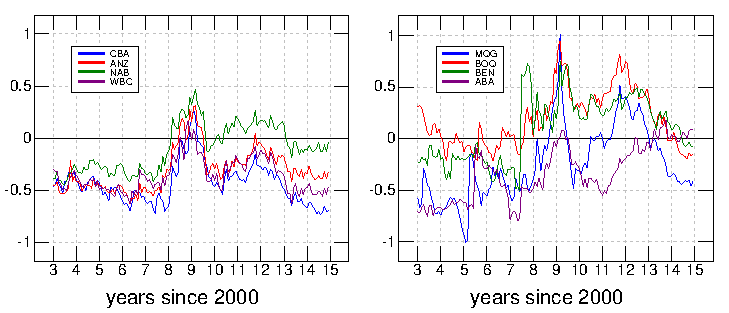
\includegraphics{figures/bloglev.pdf}
\caption{Adjusted or Basel log--leverages for four major (left panel) and four minor (right panel) Australian banks from the beginning of 2003 through to end of 2014.  All banks contravene the threshold (corresponding to the zero horizontal) around the start of 2009.}
\end{center}
\end{figure}


\section{Future capital shortfall}\label{futshort}

Financial institutions and regulators are concerned with future Basel compliance and the likelihood of a  future Basel breach.   Future compliance depends on the future return on equity.   Consider  firm $i$ at time  $t+h$ where $h>0$.  Then\footnote{In the further development $\e^\nu$ is the continuously compounded return (including principal) and $\nu$  the  rate of return or log return.}
$$
\ell_{i,t+h} = \ln \frac{d_{i,t+h}}{w_{i,t+h}} +\logit(\kappa)= \ell_{it} -\nu_{it}\cq \nu_{it}\equiv \ln\frac{w_{i,t+h}}{w_{it}}  \ ,
$$
where it is assumed $d_{i,t+h}=d_{it}$.  Here $\nu_{it}$ is the log return on equity over $(t,t+h)$ and decreases adjusted log--leverage by the same amount.  The future return is unknown at time $t$ but its probability distribution is assumed to be well understood.

The capital  shortfall  at time $t+h$, ignoring the surplus portion, is,
\be{bs}
\kappa d_{it} \left|1-\e^{-\ell_{i,t+h}}\right|^+=\kappa d_{it} \left|1-\e^{\nu_{it}-\ell_{it}}\right|^+
\cq  |x|^+\equiv \max(0,x)\ .
\ee
Thus shortfall \eref{bs} is a $\kappa d_{it}$ multiplied by a put on the return $\e^{\nu_{it}-\ell_{it}}$  with strike 1.
The Basel  limit is reached at $t+h$ if $\nu_{it}=\ell_{it}$ and  breached  if
$\nu_{it}< \ell_{it}$.
A breach is  unlikely if $\ell_{it}$ is low i.e. either the log--leverage or prudential requirement $\kappa$ is low. This paper models future capital shortfall using log return on equity $\nu_{it}$ as it is typically available publicly. An alternative approach models future asset values $d_{i,t+h}+w_{i,t+h}$ in turn implying equity returns, and is briefly discussed in \sref{riskmethod}. The risk measurement approach of this paper can be combined with any forecasting approach.


If there is a breach, $\nu_{it}<\ell_{it}$, then the amount in \eref{bs} makes up for the shortfall.   This amount may be cold comfort to regulators as it leaves the firm in a precarious position, teetering on the edge of non--compliance. Firms generally maintain a positive capital surplus to avoid breaches when unexpected shocks occur.

Default put options similar to \eref{bs} have been discussed in the insurance literature as critical to an evaluation of a firm:  see for
example \citet{merton1977analytic}, \citet{doherty1986price}, \citet{cummins1988risk}, \citet{myers2001capital} and \citet{sherris2006solvency}.

To illustrate the setup in \eref{bs}, \fref{simulation}   displays two snapshot outputs from projections generated as described  in \aref{garchdcc}:  6000  simulated one month ahead projected returns for  CBA and the market, on  two dates: the first trading day in January 2009 and the first trading day in December 2014.    Both panels use the same horizontal and vertical scales.   Thus based on the available data at those two points in  time, policy makers and regulators faced entirely different projections based on the same time series model.   The scatter of dots are the forward simulations.  Note there is no hindsight bias as the model at each time point is based on the available data to that point in time.    The red horizontal line in each panel indicates the Basel limit:  any firm return less than the limit would constitute a Basel breach.   In the left panel there is little confidence that the Basel limit will be reached since it requires a return on equity approaching 20\% -- with confidence less than xxx the Basel standard will be breached.  In the right panel there is no chance of a Basel breach under any of the projected return on equity view -- the bank is ``safe."

 The black dots in each panel indicate the actual outcome after one month.    In the left panel the outcome is a decline in both  the market and CBA stock price.    In the right panel there is slight decline in the stock price, and a more substantial market downturn.    Thus at the beginning of January  2009 CBA was projected to be far from compliance in a month while in December 2014 the one month projection is of complete compliance.

 The two panels  display very different volatility and slopes. In January 2009 both CBA and market return distributions are highly volatile and correlated. The correlation remains strong in December 2014 but with less return volatility. These snapshots are used to compute background and systemic stresses shown in subsequent sections.

\begin{figure}[htbp]
\begin{center}
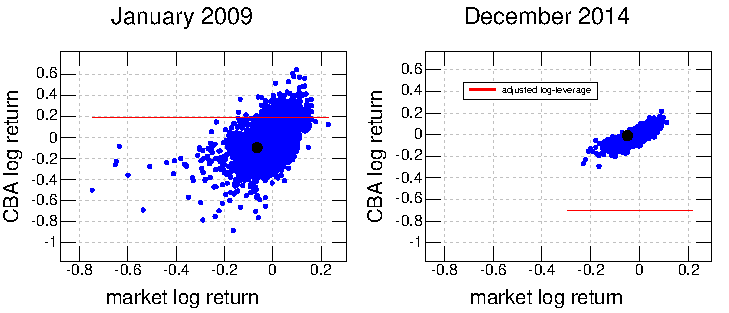
\includegraphics{figures/simulation.pdf}
\caption{Forecast bivariate distribution of one month forward rates of return   for CBA (vertical axis) and the market rate of return (horizontal axis) at start of January 2009 (left panel)  and December 2014 (right panel). Note scales in both panels are the same, the relatively large volatility in the left panel, and the left skew in the  marginal distributions.  Yellow and black dots in each panel indicate origin (0,0) and  actual forward  rate of return, respectively.   Red lines indicate Basel limit -- any firm return below the limit indicates a Basel breach given the bank leverage on the applicable date.}
\label{simulation}
\end{center}
\end{figure}

\section{SRISK and systemic risk}\label{srisk}

 \cite{brownlees2015} defines  systemic risk (SRISK) for a group of firms  at time $t$ as
\be{esrisk}
\mathrm{SRISK}_t\equiv\kappa\sum_i d_{it}\left|1-\Es(\e^{\nu_{it}-\ell_{it}})\right|^+ \ ,
\ee
where  $\Es$ denotes expectation given a major general market downturn. Hence the expected capital shortfall (allowing surplus offset) is computed from \eref{shortfall} assuming a market downturn and added across all firms. Firms having an expected capital surplus are ignored. The systemic risk of firm $i$ at time $t$ is its proportionate contribution to \eref{esrisk}:
 \be{sriskperc}
 \mathrm{SRISK}_{it}\equiv \frac{\pi_{it}|1-\Es(\e^{\nu_{it}-\ell_{it}})|^+}{\Ex_d\{|1-\Es(\e^{\nu_{it}-\ell_{it}})|^+\}}\cq \pi_{it}\equiv \frac{d_{it}}{d_t}\cq d_t\equiv \sum_i d_{it}\ ,
 \ee
where $\Ex_d$ denotes weighted averaging across firms $i$ using weights $\pi_{it}$.     Large $\mathrm{SRISK}_{it}$ indicates firm $i$ is systemically important: it holds a high proportion of the total debt, and it is likely to heavily breach the Basel capital requirement compared to remaining other firms.  Expression \eref{sriskperc} depends on $\kappa$ through each of the $\ell_{it}$.

Given a general market downturn, put values $|1-\Es(\e^{\nu_{it}-\ell_{it}})|^+$  in \eref{sriskperc} are known at time $t$:  there is no uncertainty except for possible  uncertainty in estimating the conditional  expected value.

From Jensen's inequality,
$$
\left|1-\Es(\e^{\nu_{it}-\ell_{it}})\right|^+ \le\Es\left(\left|1-\e^{\nu_{it}-\ell_{it}}\right|^+\right)\ ,
$$
with equality  if  $\nu_{it}-\ell_{it}$ is concentrated on the negative axis.  If  $\nu_{it}>\ell_{it}$  has positive probability then the  inequality is strict.   Further $\mathrm{SRISK}_{it}$ in \eref{sriskperc}   is zero whenever
$$
\ell_{it}\le \ln\Es(\e^{\nu_{it}})\ .
$$
This inequality typically holds even if the expectation conditions on an extreme market downturn. The above two inequalities suggest SRISK is not risk sensitive and leads to refinements discussed in the next section.

\section{Improved systemic risk measurement}\label{improve}

Following from \eref{bs}   define\footnote{Alternative terminology is the per unit capital shortfall put and the per unit expected capital shortfall.  For shortness we prefer the adjective Basel.  Note ``risk" here is not a probability but rather a measure of expected capital shortfall.} the  Basel put payoff and default probability of firm $i$ at time $t$ respectively as
\be{put}
p_{it}\equiv \left|1-\e^{\nu_{it}-\ell_{it}}\right|^+\cq q_{it}\equiv \p(\nu_{it}\le \ell_{it})=\frac{\E(p_{it})}{\E(p_{it}|\nu_{it}\le \ell_{it})}\ ,
\ee
where $\E$ denotes expectation without any imposed stress.  Note $0\le p_{it}\le 1$ with $p_{it}\rightarrow 0$ or 1 as $\nu_{it}\rightarrow\pm\infty$.
Further $q_{it}$ increases as the distribution of $\nu_{it}$ moves to the left.  Both $\E(p_{it})$ and $q_{it}$ measure default risk between 0 and 1, with the former reflecting the conditional distribution of $\nu_{it}$ below $\ell_{it}$ and the latter only concerned with the probability mass in the same area.


The monetary Basel put value  for firm  $i$ is the total expected payout
$$
\kappa d_{it}\E(p_{it}) = \kappa d_{it}q_{it}\E(p_{it}|\nu_{it}\le \ell_{it})\ ,
$$
the expected cost of insuring firm $i$ against a Basel breach.  The expression on the right is the product of four terms: the capital requirement $\kappa$, firm debt $d_{it}$, probability of Basel default $q_{it}$, and the expected payout if a default occurs (against a standardised exercise price of 1). In practice it may be appropriate to discount $p_{it}$ in \eref{put} by the interest rate over the period $(t,t+h)$ and value the put with risk neutral rather than normal expectation.

The put $p_{it}$ is tradable since, given $\kappa$, it relies only on the present leverage and the future return $\nu_{it}$ on equity $w_{it}$.  Market participants can value the put in  the same way as any other put and use the contract to diversify risk.  Firms can buy puts in the market to hedge their Basel default risk, or contribute an amount equal to the put value into a bailout pool.

Regulators are inclined to value the puts $p_{it}$ using a stressed, rather than risk neutral, expectation.   Stressed expectations correspond closely to conditional expectation given a system wide shock.    Regulators are concerned with the possibility and extent of Basel breaches if such shocks occur and  have an  interest in monitoring stressed expectations across firms and time.   In the extreme regulators can charge firms all or a  proportion of their stressed put values if there are implicit government bailout guarantees.



\section{Stressed expectation}

In the above development $\E$  is  unstressed expectation and does not assume a stressful scenario.   A stressed expectation, denoted $\Es$, is a
linear combination of a range of conditional expectations each assuming some level of stress:
\be{formula}
 \Es(p_{it}) \equiv \E\{\phi\E(p_{it}|\phi)\} = \E(\phi p_{it}) = \E(p_{it}) + \cov\{\E(p_{it}|\phi),\phi\}\ .
\ee
Here $\phi\ge 0$ with $\E(\phi)=1$ is a random stress factor or ``stressor,"  with different values re-weighting, and corresponding to, scenarios impacting $p_{it}$.  Thus stress $\phi$ increases the expected value $\E(p_{it})$ by the covariance between the conditional expectation $\E(p_{it}|\phi)$  and the stressor $\phi$. A larger covariance results if higher values of $\phi$, corresponding to increasingly stressed scenarios, lead to larger put values. The covariance is zero if $p_{it}$ does not vary with the different scenarios indicated by $\phi$, or under the trivial case $\phi=1$ where scenarios are not re-weighted. The impact of $\phi$ is formalised in \eref{post} below. Examples of $\phi$ implying various stress calculations are shown in subsequent sections. Weighted expectations of the form of \eref{formula} are discussed in \cite{furman2008weighted1} and \cite{choo2010determining}.

The first equality in \eref{formula} follows from the definition of conditional probability \citep{whittle2000probability}.  The second equality follows from
$$
\cov(p_{it},\phi)=\cov\{\E(p_{it}|\phi),\phi\}\ .
$$

The stressed expectation \eref{formula}  is the mean of $p_{it}$  using a stressed density
\be{post}
\int \phi f(p_{it},\phi)\de \phi= \E(\phi|p_{it})f(p_{it})\cq \int\int \phi f(p_{it},\phi)\de \phi\de p_{it} = \E(\phi) = 1\
\  ,
\ee
where $f$ denotes the density of the quantity in parentheses.
Hence the likelihood of any outcome $p_{it}$ such that $\E(\phi|p_{it})$ is large is amplified and vice versa.   To a Bayesian the density in the left  expression of $\eref{post}$ is a posterior density given a prior $f(p_{it})$ and ``likelihood" $\E(\phi|p_{it})$: more importance is given to outcomes   $p_{it}$  where $\phi$ is expected to be large.



\section{Background stress versus systemic stress}


The right hand side of \eref{formula} splits the stressed expectation $\Es(p_{it})$ into two components:
\be{vsstress}
\Es(p_{it}) =\mu_{it}+s_{it}\cq
 \mu_{it} \equiv \E(p_{it})=q_{it}\E(p_{it}|\nu_{it}\le \ell_{it}) \ ,
\ee
$$
s_{it} \equiv \cov\{\E(p_{it}|\phi),\phi\}\ ,
$$
called  the background stress  and systemic stress, respectively, in firm $i$ at time $t$. Both $\mu_{it}$ and $s_{it}$ are computed from the current adjusted log--leverage and the forward return distribution at time $t$. In addition $0\le \mu_{it},\mu_{it}+s_{it}\le 1$ and $s_{it}\ge 0$ typically holds unless firm $i$ benefits from a stress in the system. Applying a Taylor series expansion of the exponential function on $p_{it}$ yields
$$
\E(p_{it}|\nu_{it}\le \ell_{it}) \approx \ell_{it}-\E(\nu_{it}|\nu_{it}\le \ell_{it})\ ,
$$
and hence background stress decomposes into
$$
\mu_{it} \approx q_{it} \left\{\ell_{it} - \E(\nu_{it}|\nu_{it}\le \ell_{it})\right\} \ ,
$$
which is increasing in the Basel default probability $q_{it}$, adjusted log--leverage $\ell_{it}$ and the left skewness of $\nu_{it}$ as measured by the lower tail conditional expectation. If $\ell_{it}=0$  and then firm $i$ is at Basel default at time $t+h$ if  $\nu_{it}<0$ with probability $q_{it}\approx 1/2$. As  $\ell_{it}$ increases,  one month ahead Basel default becomes more certain since $\nu_{it}\le \ell_{it}$ becomes more certain and $q_{it}$ increases to 1. Background stress is unrelated to the stress factor $\phi$ and based on the unstressed distribution of the forward return $\nu_{it}$: the current view of the future progression of returns including their mean and volatility.

Similarly decompose systemic stress
$$
s_{it} = q_{\phi it}\E_\phi(p_{it}|\nu_{it}\le \ell_{it})-q_{it}\E(p_{it}|\nu_{it} \le \ell_{it})
$$
where $q_{\phi it}$ is the default probability implied from the stressed density in \eref{post}. The stress typically increases both the default probability  $q_{\phi it}$ and the conditional expected default $\E_\phi(p_{it}|\nu_{it}\le \ell_{it})$ relative to the unstressed quantities $q_{it}$ and $\E(p_{it}|\nu_{it} \le \ell_{it})$. Greater sensitivity of firm $i$ to market wide stresses leads to higher systemic stress $s_{it}$.

Monitoring $\mu_{it}$ across the market provides a leading indication of the level of background stress and anticipates buildups such as shortly before the 2008 global financial crisis. The aggregation of put values and stresses across the market is discussed and illustrated below. An increase in $\mu_{it}$ indicates either higher probabilities of defaults or larger capital shortfalls if defaults occur. Introducing systemic stress $s_{it}$ increases stress--sensitivity in two ways. Firstly adverse scenarios are emphasized which would otherwise be less obvious in $\mu_{it}$. Secondly, as $\phi$ is a market based stressor, system wide defaults and shortfalls resulting from market dependencies are emphasized and revealed.



\begin{comment}
Further
\be{mstress}
\mu_{it}=q_{it}\E(p_{it}|\nu_{it}\le \ell_{it})\ ,
\ee
where  $q_{it}$ is the Basel risk for  firm $i$  in the upcoming month,  while the second factor is the expected default size  (on a log scale)  if default occurs.
The probability $q_{it}$ depends on the  mean and volatility of daily returns at time $t$.
\end{comment}



\section{Systemic betas}

The second, systemic stress component $s_{it}$ in  \eref{vsstress}  captures the financial impact of a  hypothetical system wide financial shock.   The stress $\phi$ is systemic as it is expected to affect all firms $i$.  Further $s_{it}$ is the estimated   increase in put values on account of  $\phi$.   Examples of stress factors are given in \sref{marketstress} and \sref{genstress}.


Writing  $\sigma_{\phi}$ as the standard deviation of $\phi$,  define the systemic beta of firm $i$ with respect to stress $\phi$ as
\be{zscore}
\beta_{it}\equiv \frac{s_{it}}{\sigma_\phi} = \sigma_{it}\cor(p_{it},\phi)
\ee
where $\sigma_{it}$ is the standard deviation of $p_{it}$.   Thus $\beta_{it}$ is the systemic stress component in \eref{formula} standardised by $\sigma_\phi$ and is composed of the variability in the put payoff and its correlation with the stressor. In addition
\be{zscore2}
\Es(p_{it})  = \mu_{it} + \beta_{it}\sigma_\phi\cq \E(p_{it}|\phi) \approx \mu_{it} + \beta_{it}\frac{\phi-1}{\sigma_\phi}\ .
\ee
The second, approximate, relationship is suggested from   $\cov(p_{it},\phi)/\sigma^2_\phi$ analogous to the regression coefficient of $p_{it}$ on $\phi$.

The expressions in \eref{zscore2} suggests two ways of  thinking about the  systemic betas  $\beta_{it}$.   First, the left hand side equation shows systemic stress $\beta_{it}$ serves to shift the mean $\E(p_{it})$ of put prices  by, on average, $\sigma_\phi$.    The stress from $\phi$ is captured with $\sigma_\phi\beta_{it}$, the second term on the right of the first expression.   This term is called systemic stress and represents the addition to expected put prices if stress $\phi$ materialises.

Systemic betas are stated in terms of additions to the normal put price $\E(p_{it})$. Thus in an increasingly dire financial situation $\E(p_{it})$ will increase.   However  $\beta_{it}$ and the systemic stress measures the  change in current put values  under  further $\phi$--stress.  This varies from  \cite{brownlees2015} where $\mathrm{SRISK}_i$ does not distinguish between the current, possibly high, put prices $\E(p_{it})$ and the potential  increment due to potential stress.   Thus in an increasingly dire financial situation put prices are liable to increase on account of decreasing expected returns and increasing volatility.   However our definition of systemic stress using systemic betas measures the further effect on account of potential extra stress imposed onto the system over and above the already existing stress.   Systemic betas capture   ``marginal" effects.

The second interpretation is based on  the right hand side approximation in \eref{zscore2} showing   the change in the  expected Basel put price if  $\sigma_\phi$ units of stress $\phi$ are applied.  The quantity $(\phi-1)/\sigma_\phi$ is thought of as a ``stress factor" and is akin to the $z$--score of a normal random variable.  The stress factor has mean 0 and standard deviation 1 and is scaled by $\beta_{it}$ to yield the actual stress impact on  $p_{it}$.  Thus  $\beta_{it}$ is thought of a usual finance type ``beta" with respect to $\phi$.   Stress is measured in standardised units.  Units of stress take on different meaning depending on  $\phi$ as discussed below. The distribution of $\phi$ determines the distribution of the stress factor. If the stress factor is normally distributed then a stress effect more than doubling of the put value  occurs less than about $2.5\%$ of the time.



The  monetary stress of a firm is
$
d_{it}\beta_{it}
$
and represents the change in the monetary value of the Basel put  if stress, as captured with $\phi$, is applied.

\section{Background and systemic stress via simulation}\label{estimate}

The following computes background Stress $\mu_{it}$ and systemic stress $s_{it}$ using simulation.   Suppose $(\phi^\o,p_{it}^\o)$ are pairs of stress and put values generated from a model: for example $\phi^\o$ may be zero unless there is a market drop below the $\alpha$--percentile in which case it is $1/\alpha$.
Then
\be{simulate}
\frac{1}{N}\sum_{\o=1}^N p_{it}^\o\rightarrow \mu_{it}\cq \frac{1}{N}\sum_{\o=1}^N (\phi^\o-1)p_{it}^\o\rightarrow s_{it} \cq N\rightarrow\infty\ ,
\ee
where $N$ is the simulation effort.  The approximation is increasingly accurate as $N$ becomes large.





\section{Stress based on  market return}\label{marketstress}


The following formulates stresses as functions of the market return $\nu_{mt}$ from time $t$ to $t+h$. The examples generalise and fine--tune the approach of \cite{brownlees2015}.

\subsection{Market return below a percentile threshold}

Suppose the stress event is defined as a market return $\nu_{mt}$ in the bottom $\alpha$--tail of the distribution.   Then  $\phi(u)=1/\alpha$ for $u< \alpha$ and 0 otherwise (outcomes where $\nu_{mt}$ is better than the bottom $\alpha$--tail is ignored), and
$$
\Es(p_{it}) = \frac{1}{\alpha}\int_0^\alpha\E(p_{it}|u_{mt}=u)\de u = \E(p_{it}|u_{mt}<\alpha) = \E(p_{it}|\nu_{mt}<\tau_{t}) \ ,
$$
where $u_{mt}$ is the percentile rank of $\nu_{mt}$ and $\tau_t$ cuts out $\alpha$ probability in the lower tail of the $\nu_{mt}$ distribution: $\p(\nu_{mt}<\tau_t)=\alpha$. In addition background and systemic stresses are calculated from
$$
\mu_{it}\approx \frac{1}{N} \sum_\o p_{it}^\o \cq  \mu_{it}+s_{it}   \approx  \frac{1}{N/\alpha} \sum_{u^\o_{mt}<\alpha}  p_{it}^\o\ .
$$
The approximations decrease with the simulation effort $N$.   The effective simulation effort for $\mu_{it}+s_{it}$ or $s_{it}$ is $N/\alpha$ and hence small $\alpha$ small requires a large effort.

The threshold $\tau_t$ in the stress calculations is $F_{mt}^-(\alpha)$ where $F_{mt}^-$ is the inverse distribution function of $\nu_{mt}$. The threshold varies across time depending on market volatility, approximately $\sqrt{h}\sigma_{mt}$ where $\sigma_{mt}$ is current market volatility.   Regulators and practitioners  are well versed in working with VaR type calculations and hence a varying VaR type cutoff combining market volatility and stress is closely aligned to current practice. In comparison \cite{brownlees2015} uses fixed threshold which may be over or under extreme depending on prevailing market volatility.


\subsection{Expected worst market return in $n$ identical scenarios}

If $\phi(u)=n(1-u)^{n-1}$ then $\phi(u)\de u = \de\{1-(1-u)^n\}$ and
$$
\Es(p_{it}) \equiv \E\{\phi\E(p_{it}|\phi)\} = \int_0^1\E(p_{it}|u_{mt}=u)\de\{1-(1-u)^n\}\ .
$$
If $u$ is the market return percentile then  $1-(1-u)^n$ is the distribution of the worst percentile outcome in $n$ identical trials and hence the stressed expectation is that of the expected put price given the worst percentile market return in $n$ identical trials.  Further
$$
s_{it}  \approx  \frac{1}{N} \sum_\o \{ n(1-u^\o_{mt})^{n-1}-1\}p_{it}^\o \ .
$$
The effective simulation effort is $N/n$.
Simulated returns $\nu^\o_{mt}$ in the upper tail of the distribution  have percentiles $u^\o_{mt}\approx 1$ and hence for these market returns $(1-u^\o_{mt})^{n-1}$ is negligable and the associated simulated put $p_{it}^\omega$ is heavily downweighed.

Note the contrast with the previous example where the bottom $\alpha$ proportion of simulated market returns are selected as the stressed sample. With the current specification for $\phi$,   every simulated put contributes to the stress computation, albeit with  different weights.


\subsection{Expected worst market return given a tail event}

The above two situations can be combined.   Suppose  $\phi(u)=c(\alpha-u)^{n-1}$ for $u\le \alpha$ and 0 otherwise and where $c$ is such that $\phi(u)$ integrates to 1. Then
$$
\mu_{it}+s_{it} \approx \frac{1}{N/c}\sum_{u^\o_{mt}<\alpha}  \left(\alpha-u^\o_{mt}\right)^{n-1}p_{it}^\o\ .
$$
Similar to the first example, the stressed sample picks up the bottom $\alpha$ of market returns. The bottom $\alpha$ of market returns is further stressed by  progressively overweighing returns as the percentile approaches 0.   Large simulation effort $N$ is required for a reasonable approximation since $N/c$ is the effective simulation size and $c$ is small.


\section{Forward capital shortfall and  return simulations}\label{simulate}

The estimation of background stresses and systemic stresses and betas requires projections of future capital shortfalls. As in \cite{brownlees2015}, projections in this paper are constructed  using time series models of forward rates of return $\nu_{it}$ for firm $i$ and $\nu_{mt}$ for the market. The market return is used as the stressor with different choices of the stress function $\phi$ modelling different stress scenarios.

The time series models used are stochastic volatility models based on the GARCH--DCC model of \cite{engle2002dynamic} summarised in \aref{garchdcc}. The GARCH-DCC model captures prolonged periods of high volatility and correlation in firm and market returns, typical in financial markets. The GARCH--DCC framework is only one possible implementation.   For example future return scenarios may be constructed in a more ad--hoc manner e.g. judiciously constructed scenarios by regulators or policymakers.   The  systemic beta framework can be based on  any  generated  future  scenarios.

An earlier illustration shown in \fref{simulation} is generated from the GARCH--DCC model.  In the left panel representing one month forward returns from December 2008, low market returns are likely to lead to sharply lower CBA bank returns, as compared to the right panel showing the same as at January 2014.   This is suggested by the slope of the scatter plots:  the left slope appears steeper than the right. This implies higher systemic stress in December 2008. In addition CBA and market return volatilities are much higher in the left panel compared to the right, indicating higher background stress in December 2008. Also note that with a stressor function $\phi$ defined in terms of market return percentiles, the magnitude of a market downturn at a fixed percentile threshold is more significant in the left panel.

\begin{comment}
While the above discussion suggests, as obvious after the fact, that in December 2009 the CBA bank was under much stress.   However the above calculations do not actually reflect real stress.   In terms of the development of the previous sections the actual stress is beta given a stressor function $\phi$ and stressor variable.   In this case the stressor variable is the market return, on the horizontal axis in each panel.   Stress occurs if the market return is low.
\end{comment}

\section{One month ahead forecast stress in individual banks}\label{simulate1}

\fref{default} displays, in the top panels, the estimated $q_{it}$ one month ahead default probabilities for each major (left) and minor (right) Australian banks based on the projected one month ahead return distribution fitted using the GARCH--DCC model.  The first inclinations of Basel default arose with NAB in early 2008 followed one month later by ANZ, and  a further few months later by WBC and CBA. The probabilities subsided shortly after 2009, however NAB was close to default again in 2011 and this sustained till 2013. The volatility in default probabilities is more pronounced for smaller banks. Again note the return distributions are constructed from data only available at that time and hence are not affected by hindsight bias.

The middle two panels in \fref{default} show estimated background stress $\mu_{it}$ using the same projected return distributions. A similar pattern as default probabilities is observed, and NAB appears to have the highest put value or background stress per dollar of debt. Smaller banks are subject to higher stress in general after normalising for debt levels. Background stress levels are high across all banks around 2008 during the global financial crisis and less so between 2011 and 2013 (mainly only from NAB).


Bottom panels in \fref{default} show systemic stress $s_{it}$ computed by assuming $\phi(u)=12u^{11}$: the worst market return in 12 identical months. Systemic stress for each bank generally exhibits similar patterns as background stress $\mu_{it}$. However, importantly, some banks have differing patterns which is an important observation for the regulator since systemic stress indicates sensitivity to market-wide downturns. For example ANZ had similar systemic stress as NAB around 2012 but lower background stress. Hence although ANZ was not obviously in stress during 2012, it would be if a market downturn occurred. Bendigo and BOQ had high background stress levels after 2008, but are overtaken by Macquarie in terms of systemic risk: Macquarie is more likely to suffer in a market downturn whereas Bendigo and BOQ are less likely to be impacted.



 \begin{figure}[htbp]
\begin{center}
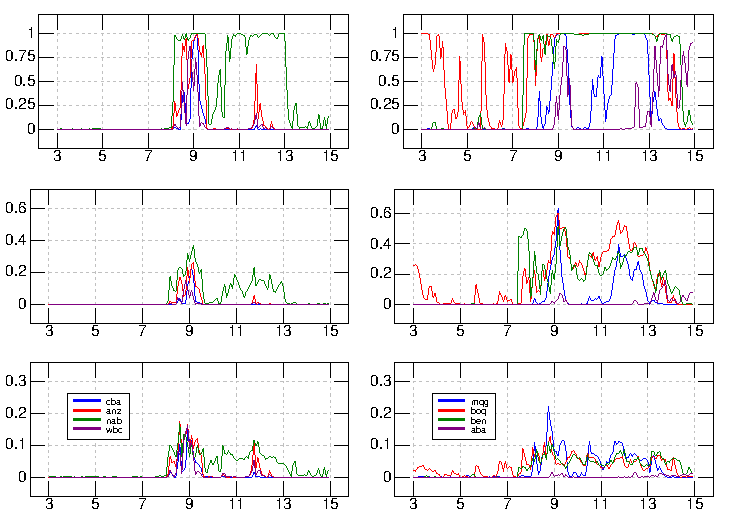
\includegraphics{figures/default.pdf}
\caption{Forecast one month ahead  Basel default probability (top panels), background stress (middle panels) and systemic stress (bottom panels) for  four major (left panel) and four minor (right panel)  banks from the beginning of 2003 through to end of 2014.  Note different scale on bottom two rows of panels.}\label{default}

\end{center}
\end{figure}


\section{Overall market stress}\label{aggregate}


There are two ways of aggregating stress in the financial market as a whole.  The first is to apply debt weighted averaging to individual firm stresses, yielding
\be{nsrisk}
\overline p_t \equiv \Exd(p_{it}) \cq \Es(\overline p_t)=\Exd\{\Es(p_{it})\} = \Exd(\mu_{it}+s_{it}) \equiv \overline\mu_{t}+\overline s_t \ ,
\ee
where $\overline\mu_{t}\equiv\Exd(\mu_{it})$ and $\overline s_{t}\equiv\Exd(s_{it})$ are overall background and systemic stresses, respectively. The put $\overline p_t$ in \eref{nsrisk} pays out zero if all firms are Basel compliant with payouts increasing with the number and size of Basel breaches. The relation in \eref{nsrisk} follow since  $\Es$ and $\Exd$ are linear.

The monetary value of overall background and systemic stresses at time $t$ are, respectively,
$$
\kappa d_t\overline\mu_t = \kappa d_t\Exd(\mu_{it}) = \kappa\sum_i d_{it}\mu_{it}\cq \kappa d_t\overline s_t  = \kappa\sum_i d_{it}s_{it}\ .
$$
Proportionate contributions of firm $i$ to background and systemic stresses are
\be{standardised}
\mu_{it}^*\equiv \frac{\pi_{it}\mu_{it}}{\overline \mu_t} \cq s_{it}^*\equiv\frac{\pi_{it}s_{it}}{\overline s_t}\ .
\ee
where $\pi_{it}\equiv d_{it}/d_t$ as before is the proportion of total debt held by firm $i$. Firm $i$ contributes to a larger portion of overall stress if it holds a large amount of debt and its returns are subject to high downside risk, particularly in a market downturn (for $s_{it}$). Contributions add to 1 across firms.  A ratio such as $s_{it}/\overline s_t$, without reflecting firm size, compares the stress in firm $i$ to average stress but does not signal the importance of that firm to the system as a whole.


\section{Overall stress after diversification}\label{aggregate1}

The debt weighed average system  put $\overline p_t\equiv\Ex_d(p_{it})$ is an average put and does not permit  diversification -- the  sharing of debt and equity across firms.   Sharing may not be possible in practice but the concept is useful for assessing the resilience of the system as a whole.   This leads to the second way of aggregating stresses across firms.

Write  $d_t$ and $w_t$ as total debt and equity in the market, respectively:
$$
d_t \equiv \sum_i d_{it}\cq w_{it} \equiv \sum_i w_{it}\ .
$$
Then the   adjusted log--leverage for the market overall is
$$
\ell_t \equiv  \ln \frac{d_t}{w_t} +\logit(\kappa) =  \ln \sum_i\frac{w_{it}}{w_t}\left(\frac{ d_{it}}{ w_{it}}\times \frac{\kappa}{1-\kappa}\right) = \ln \Ex_w(\e^{\ell_{it}}) \ ,
$$
where $\Ex_w$ denotes equity weighted averaging.  A system wide breach occurs at $t+h$ if
$
\nu_t < \ell_t
$
where $\nu_t$ is the forward rate of return on total equity $w_t$:
\be{ew}
 \nu_t =  \ln \frac{w_{t+h}}{w_t} = \ln\Ex_w\left(\frac{w_{i,t+h}}{w_{it}}\right) = \ln \Ex_w(\e^{\nu_{it}})\ .
\ee
In terms of this notation the market Basel put  and Basel risk are defined similar to \eref{put}
$$
p_t\equiv \left|1-\e^{\nu_t-\ell_t}\right|^+\le \overline p_t\cq q_t\equiv \frac{\E(p_t)}{\E(p_{t}|\nu_t<\ell_t)}=\p(\nu_t\le \ell_t) \ .
$$
The inequality is proved in  \aref{proof}.  The  put $p_t$ pays 0 at time $t+h$ unless the sector as whole is in Basel default, occurring if $\nu_t  <  \ell_t$. Moving from $\overline p_t$ to $p_t$  allows for diversification:   low liquidity  in one firm is offset by high liquidity  in other  firms.

\begin{figure}[htbp]
\begin{center}
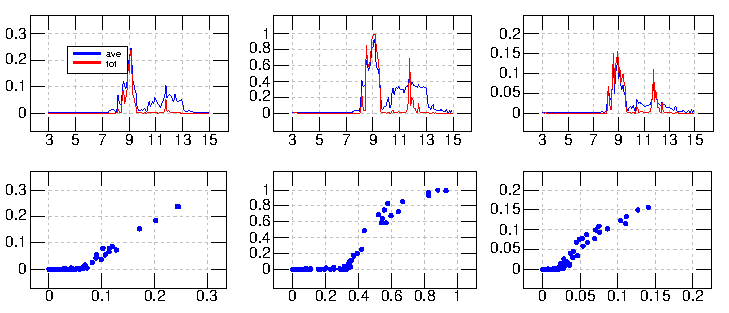
\includegraphics{figures/muqs.pdf}
\caption{Average  stresses and  total stresses.   Stress measurements are, left to right, $\mu$, $q$ and $s$, respectively.   The top row of panels measure for example (top left panel)  $\overline \mu_t$ and $\mu_t$ over time.    In the bottom row of panels  specific stresses are measured are against each other:  for example $\mu_t$ (vertical axis) versus $\overline\mu_t$ (horizontal axis).  In all cases there is no total stress until there is an appreciable level of average stress.  Systemic stress $\overline s_t$ appears to be the least diversifiable.}\label{muqs}
\end{center}
\end{figure}

Similar  to \eref{zscore2}, total  stress is decomposed as
\be{overall}
\Es(p_t) = \mu_t  + s_t\cq q_{t}=\P(\nu_t<\ell_t) \cq  s_t \equiv \cov\{\E(p_t|\phi),\phi\}\ .
\ee
termed the diversified overall background  and systemic stress, respectively.   Further $q_t$ is the probability of  a market Basel default with the second factor the expected size of the default if one occurs.

System resilience aims to answer the question of whether the system as a whole can absorb shocks.   The capacity to absorb relies on implicit merging.  When two firms merge the leverage of the resulting firm is less than that of the more highly leveraged firm.   The merged firm is more able to withstand return on equity shocks  unless negative shocks are more prone for the merged firm.   Similarly when many firms merge Basel puts for the conglomerate become less valuable.

Firms do not necessarily merge, even in dire financial circumstances.   Hence the mergers spoken of here are hypothetical.   From a regulators perspective, what would happen under a merger of all firms (or perhaps a group of firms) is nevertheless of interest.   A system as as a whole near Basel breach is more threatening that one where a few firms are near Basel breach but the system as a whole is strongly Basel compliant.

System compliance is partially monitored with the system put $\overline p_t=\Exd(p_{it})$ and its stressed expectation $\Es(\overline p_t)$. However both quantities are before diversification and give no indication of system resilience and as to how much risk can be diversified away. Basing a put on system wide aggregated debt and equity and comparing the same to $p_t$  gives at least some guidance.

\fref{muqs} compares background and systemic stresses before and after diversification. As expected, stresses reduce after diversification. The diversification is most apparent for small levels of stresses where they are close to zero. The diversification disappears when stresses reach a certain level, with points in bottom panels of \fref{muqs} following the 45$^\circ$ line. The extent of resilience or diversification over time can also be measured using the ratios $\mu_t/\overline \mu_t$ and $(\mu_t+s_t/(\overline \mu_t+\overline s_t)\le 1$. As diversification or resilience weakens such as during 2008, the ratio increases to 1.

\section{Month to month monitoring  of financial stress}\label{monitoring}
 \tref{twodates} contains real time stress calculations on the first trading day of  January 2009 and November 2014.  As before there is no look ahead bias -- all calculations on each of the two dates only use data available on the first day of the applicable month.   The initial eight rows in \tref{twodates} lists the eight banks used in this study. 
 
 \begin{table}[ht]
\caption{One month ahead bank stress calculations$^\dag$}\label{twodates}
\centering
\small
\vspace{4mm}
\begin{tabular}{l|rrrrr|rrrrr}
\hline
&\multicolumn{5}{c|}{January 2009}&\multicolumn{5}{c}{November 2014}\\
  \hline
bank & B-log& debt &\multicolumn{2}{c}{stress}&  B-def   & B-log& debt   & \multicolumn{2}{c}{stress}& B-def \\
  \cline{4-5}\cline{9-10}
       &  lev& prop    & back & syst & prob & lev& prop  & back & syst & prob \\
  \cline{2-11} 
         & $\ell_{it} $ & $\pi_{it}$ & $\mu^*_{it}$  & $s^*_{it}$ & $q_{it}$  
         & $\ell_{it} $ & $\pi_{it}$ & $\mu^*_{it}$  & $s^*_{it}$ & $q_{it}$  
        \\
  \hline
CBA & 18.57 & 24.30 & 22.99 & 29.60 & 91.43 & -70.34 & 22.70 & 0.00 & 0.00 & 0.00 \\ 
  ANZ & 15.93 & 18.37 & 14.87 & 18.89 & 92.82 & -38.64 & 22.10 & 0.00 & 0.00 & 0.00 \\ 
  NAB & 31.97 & 25.50 & 39.98 & 19.41 & 99.97 & -12.45 & 25.61 & 50.52 & 67.13 & 1.23 \\ 
  WBC & -1.55 & 22.84 & 5.86 & 23.94 & 40.42 & -53.84 & 22.03 & 0.00 & 0.00 & 0.00 \\ 
  MQG & 41.22 & 5.75 & 11.02 & 5.46 & 99.92 & -46.10 & 4.33 & 0.17 & 0.12 & 0.03 \\ 
  BOQ & 63.30 & 1.32 & 3.55 & 0.99 & 99.95 & -17.05 & 1.33 & 0.80 & 1.34 & 0.33 \\ 
  BEN & 18.91 & 1.81 & 1.72 & 1.71 & 90.53 & -7.63 & 1.84 & 25.43 & 30.71 & 8.47 \\ 
  ABA& -8.12 & 0.10 & 0.00 & 0.00 & 9.97 & 9.22 & 0.07 & 23.07 & 0.71 & 89.63 \\ 
  \hline
  $\Ex_d$ & 18.78 &  & 17.17 & 8.63 & 82.72 & -41.91 &  & 0.03 & 0.12 & 0.54 \\ 
  $\Sigma$ & 17.81 & $^\dag$2.42 & 15.28 & 10.18 & 96.72 & -44.22 & $^\dag$3.27 & 0.00 & 0.00 & 0.00 \\ 
\hline
\end{tabular}

$^\dag$All numbers multiplied by 100 except total debt (in \$bln).
\end{table}
\normalsize

January 2009 was a time of great stress for all eight banks.     The first  and second columns in the two halves of the table body contain the 
 Basel log--leverage $\ell_{it}$ and debt $\pi_{it}\equiv d_{it}/d_t$ (as a proportion of total debt) for each of the banks.  Six of the eight banks were in Basel default with positive capital shortfalls as indicated by the $\ell_{it}$ column:   the two banks not in Basel default were WBC and ABA.    Percentage background and systemic stress as defined in \eref{standardised} 
for the banks as well as the probability $q_{it}$ of a Basel default in one month are displayed in the next 3 columns.    The background stress column indicates most of the background stress arises from NAB -- almost 40\% of the total.   The next most background stressed bank is CBA with WBC also a substantial contributor.   The MQG bank contributes almost double to background stress compared to the proportion of total debt  it carries.  The other three small banks contribute relatively little to background stress with BOQ  almost 3 times expected on the basis of its debt.   Systemic stress is highest for the CBA, higher than expected on the basis of its debt load and hence CBA was most susceptible to stress from additional general market equity devaluation.    All other banks appear have systemic stress comparable to their size in terms of debt load with only NAB being less systemically important.    This should be compared to NAB's high background stress.

Continuing with January 2009, the final two rows indicate the total amount of stress in the system and it's diversifiability.    
The second last  row labelled $\Ex_d$  displays, in order, $\Ex_d(\ell_{it})$, blank, $\overline{\mu}_t\equiv \Ex_d(\mu_{it})$, $\overline{s}_t\equiv\Ex_d(s_{it})$ and  $\Ex_d(q_{it})$.   The final row labelled $\Sigma$ displays the aggregate stress quantities,treating all eight banks as one entity, $\ell_t$, total debt $d_t$ in billions of dollars,  $\mu_t$, $s_t$, and  $q_t$.
On an aggregate basis background stress is about twice systemic stress.   Thus there is more danger of increasing capital shortfall due to market volatility  as opposed to further stress from further substantial general market devaluation.  The final row indicates stresses are not diversifiable:    The marginally  smaller  ``diversified"  background stress is offset by an increase in systemic stress.    Also the diversified probability of Basel default is higher than the debt weighted average.   

Stress readings  alter dramatically when moving to November 2014 -- there is virtually no stress in any bank and the small amount of  stress in the system is diversifiable.    Most of the  background stress is carried by NAB with lesser contributions by BEN and ABA.    All the stress in the minor bank ABA is background stress as only NAB and NAB have substantial systemic stress contributions.   Again, however, it must be emphasised that there is minimal systemic stress in the system.    Only ABA has substantial Basel default probability, but this bank is a small player in the Australian banking scene.   Notice total debt in the banking sector  jumps about 35\% between the two dates.



\begin{comment}
Possible additional issues to be discussed here
\bi
\i  Usually  $q_t<\overline q_t$ reflecting diversification benefits.   However this inequality is not guaranteed since ???
$$
\Ex_d\{\P (\nu_{it}\le \ell_{it})\} \ne  \P\{\Ex_d(\nu_{it})\le \Ex_d(\ell_{it})\}
$$
\i   Comparing say $\overline s_t/s_t$ or $(\overline\mu_t+\overline s_t/(\mu_t+s_t)$ etc.   What do each of these different measures illustrate? (System robustness)
\i   Percentage measures such as  $\pi_{it}s_{it}/s_t$,  or $\pi_{it}s_{it}/(s_t+\mu_t)$.
\i  System robustness such as
\ei

\end{comment}









 \section{Generalised stress functions}\label{genstress}

Practical results for the  construction of general stress functions $\phi$ are contained in the next three subsections.


 \subsection{Stress functions as  weighted linear combinations of tail events}


\cite{brownlees2015} defines a systemic event as a market based downturn greater than a certain threshold and a systemic event  depends on the chosen threshold.   This arbitrariness is partially sidestepped by choosing a decreasing function $\phi=\phi(u_{mt})$ on the unit interval and noting
\be{wave}
\E\{\phi\E(p_{it}|\phi)\} = -\int_0^1 v\phi'(v)\E(p_{it}|u_{mt}\le v) \de v \ .
\ee
The equivalence of the left and right hand sides of \eref{wave}  follows from
$$
\int_0^1 \phi'(v)  \int_0^v \E(p_{it}|u_{mt})\de u_{mt}   \de v =\int_0^1\E(p_{it}|u_{mt})\int_{u_{mt}}^1  \phi'(v) \de v \de u_{mt}\ ,
$$
provided $\phi(1)=0$.

Thus stressed expectations, stressed with a decreasing function of the market return, is equivalent to taking a weighted average of conditional lower tail expectations.  This result is used to circumvent an explicit choice for the market threshold, replacing it with  $\phi(u)$, an implicit  mixture of thresholds.

\subsection{Scenario based stress testing}
 Stress events captured with $\phi$ and used  in \eref{zscore}  can be defined with respect any events, including a discrete number of scenarios labelled $k=1,2, \ldots$.   In this case
$$
\Es(p_{it})= \sum_k \pi_k\phi_k\E(p_{it}|k)\cq \sum_k\pi_k\phi_k = \E(\phi) = 1 ,
$$
where $\phi_k$ is the weight assigned to scenario $k$ and $\pi_k$ here is the original probability of scenario $k$.   The $\pi_k\phi_k\ge 0$ are  modified  probabilities which weigh different scenarios according to level of interest.   For example in standard stress testing the $\phi_k$ are chosen such that significant weight is given to scenarios causing high  firm distress.   The ``real world" probabilities $\pi_k$ are  usually ignored by  simply choosing  $\pi_k\phi_k$ to be of  required magnitude.

In the discrete case $s_{it}$ compares the expected value under an average of distress scenarios to the average without distress.  The quantity $\sigma_\phi$ is now of limited relevance, signalling the volatility in the distress probabilities.


\subsection{Copula stress functions}


Stress can be based on a vector of variables $x$ with marginal distributions $F$ and marginal densities $f$. The vector of percentile ranks corresponding to $x$ is $u=F(x)$.  Suppose $c$ is the copula density of $x$ implying the joint density of $x$ is $c(u)\prod_jf(x_j)$.    If   $\phi(u)$ is a copula stress density where $\E\{\phi(u)\}=1$ then the stressed expectation of the put is
\be{copula}
\Es(p_{it}) \equiv \int \E(p_{it}|x)\phi(u)c(u)\prod_j\{f(x_j)\}  \de x   \ .
\ee
If $\phi(u)=1$  then $\Es(p_{it})=\E(p_{it})$, the ordinary expectation.   The density $\phi(u)$ magnifies potentially stressful situation such as where all components of $x$ are distressed (either high or low depending on each component of $x$).

The copula density stressor $\phi(u)$  can be combined with marginal stressors written as functions of $x_j$ or  percentiles $u_j$.  If the latter then $\phi(u)\prod_j\psi_j(u_j)$ is the total stressor which is applied to $\E(p_{it}|x)$ as above.

Copula stress effects are simulated as follows.   Suppose $x$ is a vector $\nu_{mt}$ of  market factors  over the period $(t,t+h)$.   Simulations of a joint model are  used to  compute vectors $(p_{it}^\o,\nu_{mt}^\o)$, $ \o=1,\ldots, N$.  The $\nu_{mt}^\o$ are  converted to percentiles $u^\o$ and scalars
$$
\phi^\o\equiv\phi(u^\o)\prod_j\psi_j(u_j^\o)\cq \o=1,\ldots, N\ ,
$$
are calculated. The systemic stress and beta are then estimated as in \eref{simulate}.



\section{Modelling assets to determine capital shortfall}\label{riskmethod}

An alternative method to determine capital adequacy is to value  assets separately, apply the prudential requirement and subtract debt to arrive at capital shortfall.   The capital shortfall at time $t+h$ is then, similar to \eref{shortfall},
\be{csrwa}
d_{it} - (1-\kappa)\sum_j \e^{\nu_{ijt}}a_{ijt}  = d_{it} - (1-\kappa)a_{it}\Ex_a(\e^{\nu_{ijt}})\cq a_{it}=\sum_j a_{ijt}\ .
\ee
Here $a_{ijt}$ is the value of firm $i$'s asset  $j$ at time $t$ and has forward log--return $\nu_{ijt}$.  Further  $\Ex_a$ denotes an asset weighted average using  firm $i$'s asset values at time $t$. The default put is, per unit $\kappa d_{it}$,
\be{modput}
p_{it}\equiv \left|k^{-1} - \e^{-\logit\kappa-L_{it}}\Ex_a(\e^{\nu_{ijt}})\right|^+ \cq L_{it}\equiv \ln\frac{d_{it}}{a_{it}} \ .
\ee
Thus $\e^{L_{it}}$ is the often used alternative leverage definition: dividing debt by total assets.   Similar to before $0\le p_{it}\le 1$ is a measure of  stress on firm $i$ at time $t$ with total stressed expectation decomposed as before:
$$
\Es(p_{it}) = \E(p_{it}) + \cov\{\E(p_{it}|\phi),\phi\} = \mu_{it} + s_{it}\ ,
$$
where $\mu_{it}$ is the background stress and $s_{it}$ is the systemic stress, i.e. the result of systemic event modelled with $\phi$.

To calculate put values or stresses as before, a sample of $N$ forward returns $\nu_{ijt}^\o$ and stress factors $\phi^\o$ are  simulated using an appropriate model such as the GARCH--DCC model.   The returns $\nu_{ijt}^\o$ are used to derive $\Ex_a(\e^{\nu_{ijt}^\o})$ and in turn, using \eref{modput},   $p_{it}^\o$ which are multiplied by $\phi^\o$ to arrive at stressed put prices  $\phi^\o p_{it}^\o$.  The calculations converge as $N\rightarrow\infty$:
\be{rwa}
\frac{1}{N}\sum_\o \phi^\o p_{it}^\o\rightarrow \Es(p_{it})\cq \Ex_a\left( \frac{1}{N}\sum_\o\phi^\o\e^{\nu_{ijt}^\o}\right)\rightarrow \Es\{\Ex_a(\e^{\nu_{ijt}})\}\ .
\ee

Note that
$$
\Es(p_{it}) \ne \left|k^{-1}-\e^{-\logit\kappa-L_{it}}\Es\{\Ex_a(\e^{\nu_{ijt}})\}\right|^+\ .
$$
The stressed average return
$$
\Es\{\Ex_a(\e^{\nu_{ijt}})\} = \Ex_a\{\Es(\e^{\nu_{ijt}})\} \approx \Ex_a\left( \frac{1}{N}\sum_\o\phi^\o\e^{\nu_{ijt}^\o}\right)\ ,
$$
cannot be used directly in the calculation of firm stress.

An easily stressed asset $j$  has a return distribution sensitive to stresses or changes in values of $\phi$. Under stress, $\e^{\nu_{ijt}}$ is likely to be much less than 1 thus increasing the capital shortfall. This asset increases the stressed expectation of $p_{it}$ particularly when $a_{ijt}$ contributes to large portion of $a_{it}$.







\section{Background and systemic stress  compared to SRISK}\label{comparison}

The methodology developed and employed in this article departs in three respects from the SRISK methodology set out in \cite{brownlees2015}.  This section examines the force of these differences.

\subsection{Put value versus put on expected value}

The SRISK methodology described in \sref{srisk}, in particular \eref{sriskperc}, is based on a put on the expected shortfall:
\be{prisk}
 |1-\E_\phi(\e^{\nu_{it}-\ell_{it}})|^+\le \Es(|1-\e^{\nu_{it}-\ell_{it}}|^+) \equiv \mu_{it}+s_{it}\ ,
\ee
where stressed expectation $\Es$ in \cite{brownlees2015} is conditional expectation given a major market downturn.  The   put is evaluated after the expectation $\Es$ and checks, in essence whether in a significant market downturn, the expected $h$ period ahead return $\nu_{it}$ exceeds the adjusted   log--leverage.  If this holds true there may still be substantial risk of a Basel breach, depending on the volatility of the return.   Volatility in $\nu_{it}$ is ignored in  $\mathrm{SRISK}_{it}$  other than through the usual adjustment on account of continuous compounding.  In particular increased volatility due to stress is ignored.

With the proposed $\mu_{it}+s_{it}$ where the stressed expectation is performed on the put payoff as opposed to the other way round, return volatility is taken into consideration as for any other puts in general. Other things equal, higher volatility leads to higher put values since breach size is taken into consideration. An explicit decomposition is discussed in \sref{improve}. In addition the calculation by \cite{brownlees2015} has a probability mass at the zero value whereas the proposed calculation yields a continuous range of values unless a breach is highly unlikely.


\begin{comment}
Note further we split up $\mu_{it}=q_{it}\E(p_{it}|\nu_{it}>\ell_{it})$.    (Can do analogous split up on $s_{it}$ ????)

(Should we compare $\mu_{it}+s_{it}$ to the left  hand side of $\eref{prisk}$ using graphs???)
\end{comment}


\subsection{Systemic stress versus background stress}

\cite{brownlees2015} defines systemic risk as the entire left of \eref{prisk}. However a stressed expectation may be high simply on account of put prices already being high before stressing, reflecting higher than normal volatility or leverage. Hence \cite{brownlees2015} combines both background stress, due to high volatility or leverage, and the imposed system stress. However it is important to understand the mix of the two different stresses. \fref{sysstress} plots systemic stress versus background stress for the eight Australian banks of \tref{banks}.   Generally background stress is higher than systemic stress, although the mix differs between banks and the extent of stress. For example compared to the smaller Australian banks, bigger banks have a larger proportion of systemic stress relative to background stress. In addition Macquarie is more systemically risky amongst the smaller banks.



\begin{comment}
To gain insight into the relative sizes of these two components, consider the proportion of the stressed put price due to a possible future stress scenario
$$
\frac{\Es(p_{it})-\E(p_{it})}{\Es(p_{it})} = \frac{\sigma_\phi\beta_{it}}{\mu_{it}+\sigma_\phi\beta_{it}}  \ .
$$
The denominator is total stress in firm $i$, made up of two components:   the volatility stress $\mu_{it}=\E(p_{it})$ and the systemic stress $\sigma_\phi\beta_{it}=\Es(p_it)-\E(p_{it})$.   Volatility stress  arises on account  of high volatility in the markets causing high put prices.   Systemic stress is the additional stress caused by  a potential  bad systemic event.
\end{comment}

\begin{figure}[htbp]
\begin{center}
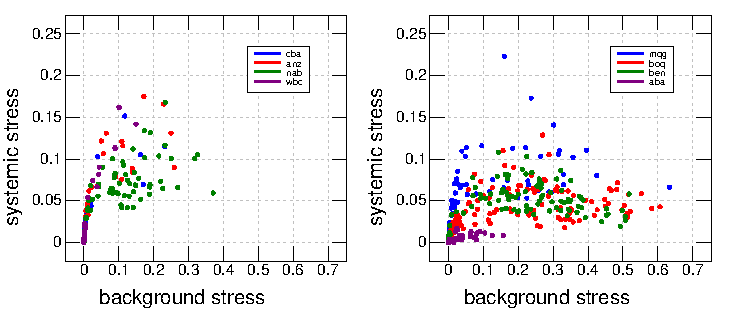
\includegraphics{figures/sysstress.pdf}
\caption{Systemic, $s_{it}$, versus background $\mu_{it}$   for four major banks (left panel) and four minor banks (right panel)  for 144 months.}
\label{sysstress}
\end{center}
\end{figure}


\subsection{Flexible  stress  functions}

The further modification made to the SRISK methodology of \cite{brownlees2015} is to generalise the ``cutoff" functional form for stressing.   With the latter, stressed expectations are conditional expectations given a specified cutoff point.  For SRISK in \cite{brownlees2015} the cutoff is in absolute terms:  a 10\% fall in the market although this can varied.   This cutoff does not allow for market volatility:   a 10\% reduction is  increasingly plausible as volatility increases.  In addition  SRISK does not  make judgement as to the likelihood of the conditioning stress event.   Thus SRISK mixes in various  sources of risk in an imprecise manner and it is difficult to determine the implications of SRISK readings.

This argues for specifying conditional behaviour in percentile terms relative to the then applicable market conditions, as in done in this paper.  After all, current market volatility is known and there is a good reason to disentangle current market conditions from the evaluation of what is likely to happen if further stress arrives in the system.

Stresses are further generalised in this paper with generalized univariate and multivariate forms of $\phi$, as well as discrete forms of $\phi$ which are aligned with the widespread approach of stress testing to measure individual firm and systemic risk by APRA and other prudential regulators.



\section{Conclusion}\label{conclude}


This paper develops an approach to measure systemic risk using the concept of stressed expectations which formalise stress testing widely used in practice. Systemic stress adds to background stress which is the value of default puts on firms. Fitting time series to Australian bank data identifies banks previously in distress and those with high contribution to systemic risk.


\begin{comment}



\section{Application to Australian financial institutions}

 (have to merge this with other stuff elsewhere)

At each of the first trading day in the months from January 2003 through to December 2014,  all prior returns are used estimate a TARCH-DCC model described below.   For each first trading day of the month, the fitted model is then used to simulate the forward return distribution over the next 22 trading days, corresponding to approximately one month.  The details of the fitted models are described in the next subsection.


\subsection{Forward return simulation}

The forward simulations are implemented similar to \cite{brownlees2015}.   Given the latest available volatility and correlation estimates the filter recursions are moved forward in time using innovations randomly chosen from past standardised innovations.  Thus the innovations are chosen to have the same marginal distributions as applicable in the past.  The random choices are such  that the same market return innovations are used in each bivariate analysis.



\section{Comparing SRISK for different firms (not sure)}

Suppose of interest is whether $\beta_{it}$ varies similarly  across firms as $\tau$ varies where $\tau$ is the threshold, $\kappa$, or some other parameter used to compute $\beta_{it}$. High correlation implies high systemic risk since firms are simultaneously affected.

Define $\eps_{it}\equiv(\phi-1)p_{it}$ and $\eps_{it}$ as the vector with components $\eps_{it}$.  Then $\E(\eps_{it}|\tau)=\sigma_\phi(\tau)\beta_{it}(\tau)$, the stress in firm $i$ at the given parameter setting $\tau$  and
$$
\cov\{\E(\eps_{it}|\tau)\}=\cov(\eps_{t})-\E\{\cov(\eps_{it}|\tau)\}\ ,
$$
is the covariance between stresses as $\tau$, the stress parameter varies.   Thus the covariances and correlations between firms as stress parameters vary can be computed from the covariability between the $\eps_{it}$ and the ...


\subsection{Weihao - Allocating the market put}

The overall market shortfall after allowing for diversification between firms is
$$
p_{mt}\equiv k_+ |1-\e^{-\ell^*_{mt}+\nu_{mt}}|^+
= k_+|\Ex (1-\e^{-\ell^*_{it}+\nu_{it}})|^+
=I(\nu_{mt}<\ell_{mt}^*)k_+\Ex(1-\e^{-\ell^*_{it}+\nu_{it}})
$$
and hence the portion attributable to firm $i$ is $k_i(1-\e^{-\ell^*_{it}+\nu_{it}}) I(\nu_{mt}<\ell_{mt}^*)$, its capital shortfall or surplus when the overall market is in a shortfall. The allocation of the stressed expectation $\E(p_{mt})$ is then
$$
k_i\E\{(1-\e^{-\ell^*_{it}+\nu_{it}}) I(\nu_{mt}<\ell_{mt}^*)\}
$$
and applying $\Ex$ to the above expression yields $\E(p_{mt})$.
\end{comment}


\bigskip
\begin{center}
{\large\bf SUPPLEMENTARY MATERIAL}
\end{center}

\appendix
\renewcommand*{\thesection}{\Alph{section}}

\section{GARCH--DCC model}\label{garchdcc}

Denote the daily (log) return for firm $i$ at time $t$ as
\newcommand{\vareps}{\varepsilon}
\be{mean.model}
\delta_{it}=\mu_i+\sigma_{it}\eps_{it}\cq \eps_{it}\sim (0,1)\ ,
\ee
The volatility $\sigma_{it}$ is modelled as
\be{vol}
\sigma_{i,t+1}^2 = \omega+ \sigma^2_{it}\{\beta+(\alpha+\gamma \eps^-_{it})\eps_{it}^2\}  \cq  \eps^-_{it}\equiv I(\eps_{it}<0)=I(\delta_{it}<\mu)\ .
\ee
where $I$ denotes the indicator function.  Hence the response of $\sigma_{i,t+1}^2$ to $\eps_{it}^2$  is increased by $\gamma$   if
the rate of return is below the average $\mu_i$, compared to the response if $\delta_{it}>\mu_i$.  Equations \eref{mean.model} and \eref{vol} defined a simple threshold GARCH model:  called the TARCH(1,1).   In \eref{mean.model} the mean $\mu_i$ does not vary with time $t$ and in \eref{vol} it is assumed the terms  $\sigma_{it}^2$ and $\eps_{it}$ in the right hand side of \eref{vol} are sufficient to structure the dynamics of volatility.

The model defined by \eref{mean.model} and \eref{vol} is estimated  for each security $i$ jointly with  a similar model for  the market,  $i=m$.   The correlations between securities and the market are modelled using  positive definite recursions   \citep{engle2002dynamic}
$$
(Q_{i,t+1}-S) = \alpha (\eta_{it}\eta_{it}'-S) + \beta (Q_{it}-S)\cq \eta_{it}\equiv(\eps_{it},\eps_{mt})' .
$$
Correlations $\rho_{it}$ recovered from the $Q_{it}$ are used as the correlation between $\eps_{it}$ and $\eps_{mt}$.

\section{Proof of system put is less   than debt weighted average put}\label{proof}
Since
$$
1-\e^{-\ell_{it}} = \frac{ \kappa d_{it} - (1-\kappa)w_{it}}{\kappa d_{it}}\cq \Ex_d (1-\e^{-\ell_{it}}) = \frac{\kappa d_t - (1-\kappa) w_t}{\kappa d_t} = 1-\e^{-\ell_t} \ ,
$$
and similarly if $-\ell_{it}$ is replaced by $\nu_{it}-\ell_{it}$.   Hence
$$
p_t\equiv |1-\e^{-\ell_t}|^+ \le \Ex_d (|1-\e^{-\ell_{it}}|^+)\equiv \overline p_t\ .
$$

\section{Use of more general puts}

Consider the put $p_{it}(1+cp_{it})=p_{it}+cp_{it}^2 $ for some constant $c\ge 0$.   This put is zero if $p_{it}=0$ and has slope $1+2cp_{it}$ for $p_{it}>0$ and $p_{it}(1+cp_{it})>p_{it}$ if the put is positive.  Larger slopes $c$ imply greater payoff.

The put $p_{it}+cp_{it}^2$ imposes a higher cost structure on defaults.    For every extra dollar of default the cost increases by $1+2cp_{it}$.   Further the stressed put value is
$$
\E(p_{it})\left\{1+c\E(p_{it})\right\} +c\left\{\cov(p_{it})\right\}+ \cov(p_{it},\phi) + c\left\{\cov(p^2_{it},\phi)\right\}
$$
$$
=\E(p_{it})\left\{1+c\E(p_{it})\right\} +c\left\{\cov(p_{it})\right\}+ \cov(p_{it}+cp^2_{it},\phi)\ .
$$
The first three terms in the final expression are unrelated to stress $\phi$: stress only impacts the last term.

\section{Data sources}\label{data}

Data are sourced from DataStream. DataStream company codes are 
\begin{center}
	\begin{tabular}{ll}
A:ANZX & Australia and New Zealand Banking Group Limited\\
A:ABAX & Auswide Bank Limited\\
A:BOQX & Bank of Queensland Limited\\
A:BENX & Bendigo and Adelaide Bank Limited\\
A:CBAX & Commonwealth Bank of Australia\\
A:MQGX & Macquarie Bank Limited\\
A:NABX & National Australia Bank Limited\\
A:WBCX & Westpac Banking Corporation.\\	
\end{tabular}
\end{center}

DataStream datatype codes are
\begin{center}
	\begin{tabular}{ll}
	NOSH & Number of Shares\\
	P & Price\\
	WC02999 & Total Assets\\
	WC03501 & Shareholders Equity\\
	RZ & Total return index\\
\end{tabular}
\end{center}

Firm equity $w_{it}$ is Number of Shares multiplied by Price. Firm debt $d_{it}$ is Total Assets minus Shareholders Equity. Stock returns are computed from the Total Return Index which includes dividends as paid. 

\section{Computations}

All model fits in this paper are performed with the R language \citep{R-Development-Core-Team:2008aa} and in particular the rmgarch package described by \cite{ghalanos2012rmgarch}.  All other calculations are done in the J language \citep{iverson2003j}.

In the forward simulated forward projections the  innovations are chosen randomly from past innovations.   These past innovations are chosen consistently:  at a particular $t$ either all or none of $\eps_{it}$ are chosen.




\bibliography{piet2}
\end{document}
